\documentclass[a4paper,12pt]{article}

%% Language and font encodings
\usepackage[english, russian]{babel}
\usepackage[utf8x]{inputenc}
\usepackage{blindtext}
\usepackage[T1]{fontenc}
\usepackage[T2A]{fontenc}
\usepackage[a4paper,top=1.5 cm,bottom=2cm,left=3cm,right=3cm,marginparwidth=1.75cm]{geometry}
%% Useful packages
\usepackage{amsmath, amssymb}
\usepackage{wrapfig}
\usepackage{graphicx}
\usepackage[usenames]{color}
\usepackage[T1]{fontenc}
\usepackage{tikz}
\usetikzlibrary{arrows}
\usetikzlibrary{decorations.pathreplacing}
\usepackage[T2A]{fontenc}
\usepackage{color}
\usepackage{circuitikz} 
\graphicspath{{pic/}}
\definecolor{water} {rgb} {0.667, 0.855, 1}
\usepackage{pgfplots}
\usepackage{pgfplotstable}
\usetikzlibrary{circuits}
\usetikzlibrary{circuits.ee}
\usetikzlibrary{circuits.ee.IEC}
\usetikzlibrary{circuits.logic.IEC}
\usetikzlibrary{intersections}

\title{ДИФРАКЦИЯ СВЕТА НА ЗВУКОВОЙ ВОЛНЕ В ЖИДКОСТИ}
\date{Работа 4.3.2A}
\author{Пазов Тенгиз, Симухин Егор, группа Б03-302}
\begin{document}
		\vspace{0.5 cm}
	\maketitle
	\vspace{0.5 cm}
	
	\textbf{Анотация:} 1) В работе изучается дифракция света на синусоидальной акустической решетке и наблюдается фазовая решетка.
Измеряется длина волны ультразвука и скорость ультразвука в воде.
2) В работе используются оптическая скамья, осветитель, два длиннофокусных объектива, кювета с жидкостью, кварцевый излучатель с микрометрическим винтом, генератор звуковой частоты, линза, горизонтальная нить на рейтере, микроскоп.
	
	\section*{Теоретическое введение}
При прохождении ультразвуковой волны через жидкость в ней возникают периодические неоднородности коэффициента преломления, создается фазовая решетка, которую мы считаем неподвижной ввиду малости скорости звука относительно скорости света. Показатель
	преломления n изменяется по закону:
	
	\begin{equation}\label{}
	n = n_0 (1 + m \cos \Omega x)
	\end{equation}
	
	Здесь $ \Omega = 2 \pi / \Lambda $ --- волновое число для ультразвуковой волны, $ m $ --- глубина модуляции $ n $ $ (m \ll 1 $).
	
	Положим фазу $ \phi $ колебаний световой волны на передней стенке кюветы равной нулю, тогда на задней поверхности она равна:
	
	\begin{equation}\label{}
	\phi  = k n L = \phi_0 (1 + m \cos \Omega x)
	\end{equation}
	
	Здесь $ L $ --- толщина жидкости в кювете, $ k = 2 \pi / \lambda $ --- волновое число для света.
	
	После прохождения через кювету световое поле есть совокупность плоских волн, распространяющихся под углами $ \theta $, соответствующими максимумам в дифракции Фраунгофера:
	
\begin{equation}\label{}	
	\Lambda \sin \theta_m = m \lambda
\end{equation}

	Этот эффект проиллюстрирован на рисунке 1.
	\begin{figure}[h!]
		\centering	
		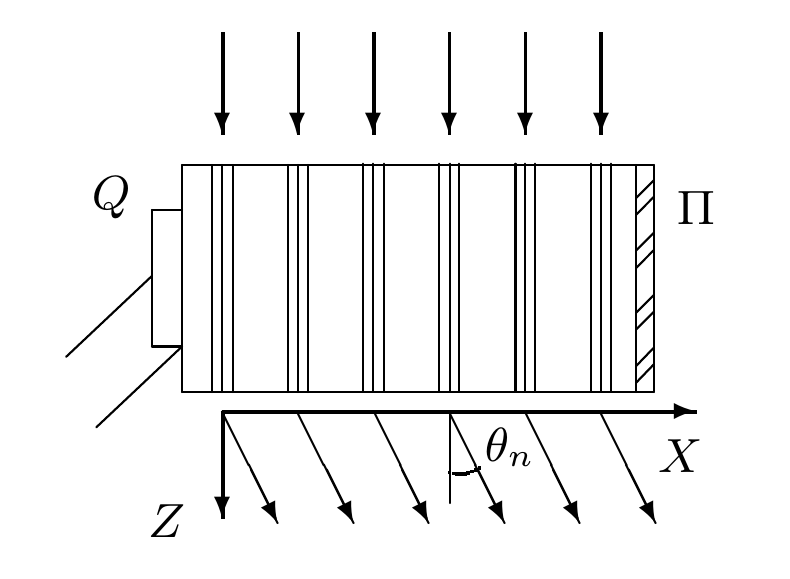
\includegraphics[width=0.3\textwidth]{difraction.png}
		\caption{Дифракция световых волн на акустической решетке}
		\label{diff}
	\end{figure}
    Зная положение дифракционных максимумов, по формуле (1) легко определить длину ультразвуковой волны, учитывая малость $ \theta $: $ \sin \theta \approx \theta \approx l_m /F  $, где $ l_m $ --- расстояние от нулевого до последнего видимого максимума, $ F $ --- фокусное расстояние линзы. Тогда получим:
    	
    	\begin{equation}\label{}
    	 \Lambda = m \lambda F/ l_m 
    	\end{equation}
    	Скорость ультразвуковых волн в жидкости, где $ \nu $ --- частота колебаний излучателя:
    	
    \begin{equation}\label{}
    	v = \Lambda \nu 
    \end{equation}
    
   
	\section*{Методика измерений}
Используются следующие методы изучения дифракции:\\
2.1.)Метод определения длины волны по дифракционной решетке, основанный на построении графика $x_{m}(m)$(положения диффракционных максимумов от номера максимума), чтобы по формуле (4) найти длину волны.\\ 
2.2.) Метод измерения скорости ультразвука в воде по коэффициенту наклона графика $\Lambda (\frac{1}{\nu})$.\\
2.3.) Метод темного поля, заключающийся в устранении центрального дифракционного максимума с помощью специального экрана(проволочки).\\
 \textbf{Схема установки. }Схема установки приведена на рисунке 2. Источник света Л через светофильтр Ф и конденсор К освещает вертикальную щель $ S $, находящуюся в фокусе объектива $ O_1 $. После объектива параллельный световой пучок проходит через кювету С перпендикулярно акустической решетке, и дифракционная картина собирается в фокальной плоскости объектива $ O_2 $ , наблюдается при помощи микроскопа М.

    Предварительную настройку установки произведем в соответствии с инструкцией с зеленым фильтром, далее в работе используется красный.
    
    	\begin{figure}[h!]
    	\centering	
    	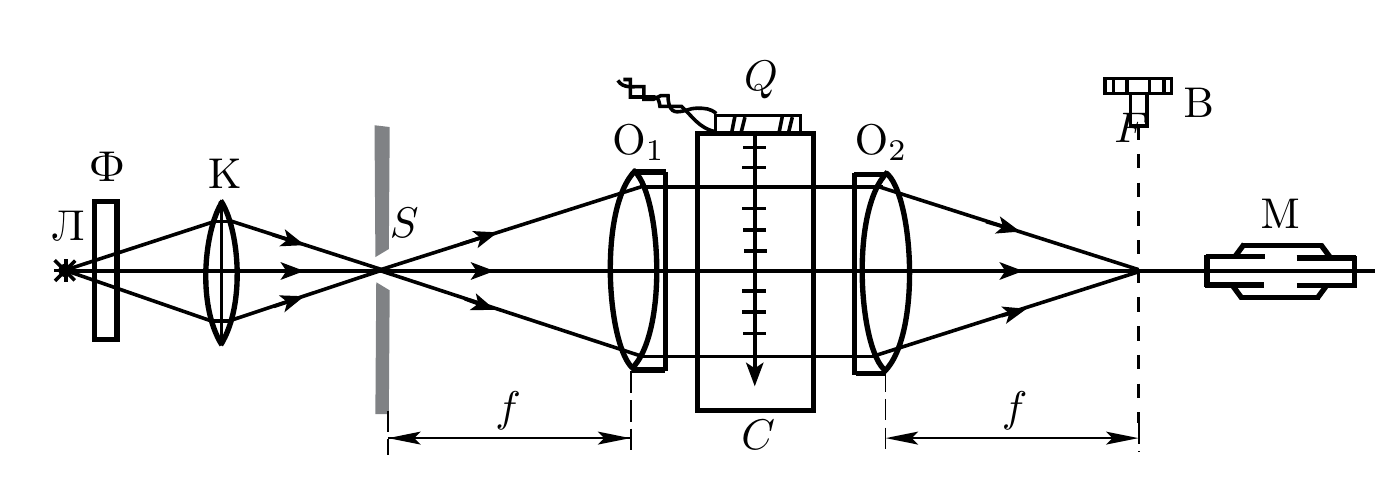
\includegraphics[width=0.7\textwidth]{shema1.png}
    	\caption{Схема для наблюдения дифракции на акустической решетке}
    	\label{shema1}
    \end{figure}
    
    Параметры установки: фокусное расстояние объектива $F = 30 $ см, одно деление винта микроскопа составляет 20~мкм, полоса пропускания фильтра \mbox{$\lambda = 6400\pm 200$ Å}.\\
    \textbf{Оборудование и инструментальные погрешности}.\\
    Погрешность микрометрического винта(отсчётного устройства): 0.01мм(ввиду жесткой болтанки).\\
    Погрешность микриметрического винта(излучателя): 0.01мм.
	\section*{Результаты измерений}
	\begin{enumerate}
	    \item Исследовали изменения дифракционной картины на красном свете. При увеличении частоты УЗ-генератора и приближении к 1,1~МГц проявляется дифракционная решетка: расстояние между максимумами растет.
	    
	    Измерили положения $ x_m $ дифракционных максимумов с помощью микроскопического винта для пяти частот. Для каждой полосы измерили крайние координаты и рассчитали среднее относительно нулевого максимума как координату полосы. Результаты измерений занесли в таблицах ниже. На основе каждой таблицы построили графики зависимости $ x_m (m) $.
	    
	    1. Для частоты $\nu_1=1{,}0116\pm 0{,}0001$ МГц:
	    \begin{center}
	    \begin{tabular}{|c|c|c|c|c|c|c|c|c|}
            \hline
            $m$ & -3 & -2 & -1 & 0 & 1 & 2 & 3 & 4 \\ \hline
            $x_m$, дел. & 2,225 & 2,50 & 2,80 & 3,10 & 3,425 & 3,70 & 3,975 & 4,275 \\ \hline
            $x_m$, мкм & -350 & -240 & -120 & 0 & 130 & 240 & 350 & 470 \\ \hline
        \end{tabular}
	    \end{center}
	\item Для частоты $\nu_2=1{,}2092\pm 0{,}0001$ МГц:
	    \begin{center}
	    \begin{tabular}{|c|c|c|c|c|c|c|c|}
            \hline
            $m$ & -3 & -2 & -1 & 0 & 1 & 2 & 3 \\ \hline
            $x_m$, дел. & 2,05 & 2,40 & 2,75 & 3,10 & 3,475 & 3,775 & 4,125 \\ \hline
            $x_m$, мкм & -420 & -280 & -140 & 0 & 150 & 240 & 410 \\ \hline
        \end{tabular}
	    \end{center}
	    

	
	\item Для частоты $\nu_3=2{,}9332\pm 0{,}0001$ МГц:
	    \begin{center}
	    \begin{tabular}{|c|c|c|c|c|c|c|c|}
            \hline
            $m$ & -2 & -1 & 0 & 1 & 2 & 3 \\ \hline
            $x_m$, дел. & 1,425 & 2,30 & 3,10 & 3,925 & 4,80 & 5,625 \\ \hline
            $x_m$, мкм & -670 & -320 & 0 & 330 & 680 & 1010 \\ \hline
        \end{tabular}
	    \end{center}

	
	\item Дальше резонансы получать всё сложнее, к тому же в поле обзора попадает меньше полос либо полосы второго порядка не возникают. Графики по трём точкам строить бессмысленно. Для частоты $\nu_4=4{,}6086\pm 0{,}0001$~МГц:
	    \begin{center}
	    \begin{tabular}{|c|c|c|c|}
            \hline
            $m$ & -1 & 0 & 1 \\ \hline
            $x_m$, дел. & 1,775 & 3,10 & 4,425 \\ \hline
            $x_m$, мкм & -530 & 0 & 530 \\ \hline
        \end{tabular}
	    \end{center}
	\item Для частоты $\nu_5=5{,}1911\pm 0{,}0001$ МГц:
	    \begin{center}
	    \begin{tabular}{|c|c|c|c|}
            \hline
            $m$ & -1 & 0 & 1 \\ \hline
            $x_m$, дел. & 1,625 & 3,10 & 4,60 \\ \hline
            $x_m$, мкм & -590 & 0 & 600 \\ \hline
        \end{tabular}
	    \end{center}
	\end{enumerate}
	\section*{Обработка результатов}
	\begin{figure}[h!]
		\centering	
		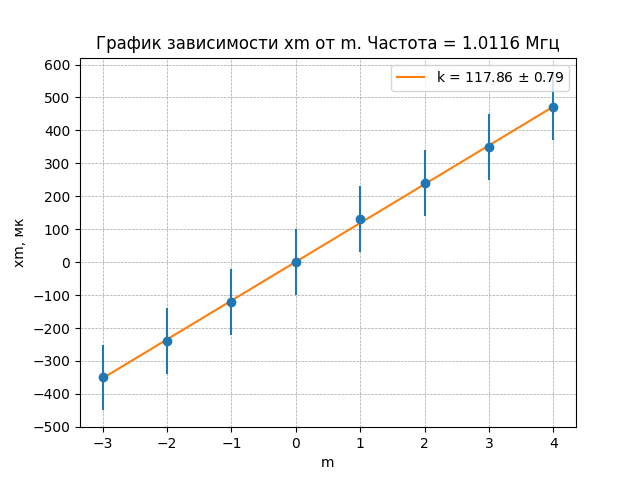
\includegraphics[width=1\textwidth]{1.png}
		\caption{График зависимости $x_{m}(m)$ при $\nu_{1}$}
		\label{diff}
	\end{figure}
	\begin{figure}[h!]
		\centering	
		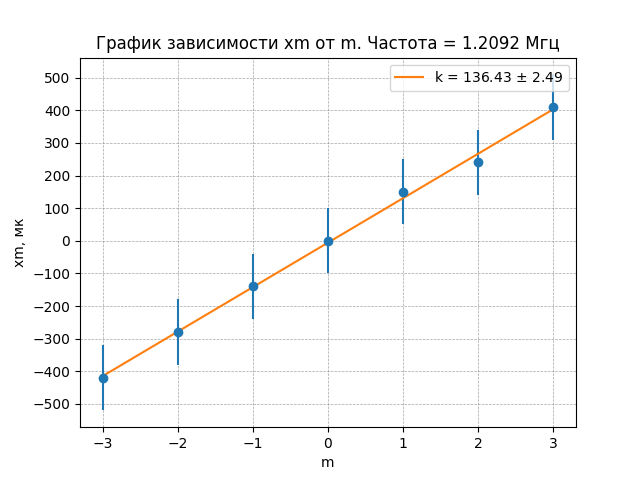
\includegraphics[width=1\textwidth]{2.png}
		\caption{График зависимости $x_{m}(m)$ при $\nu_{2}$}
		\label{diff}
	\end{figure}
	\begin{figure}[h!]
		\centering	
		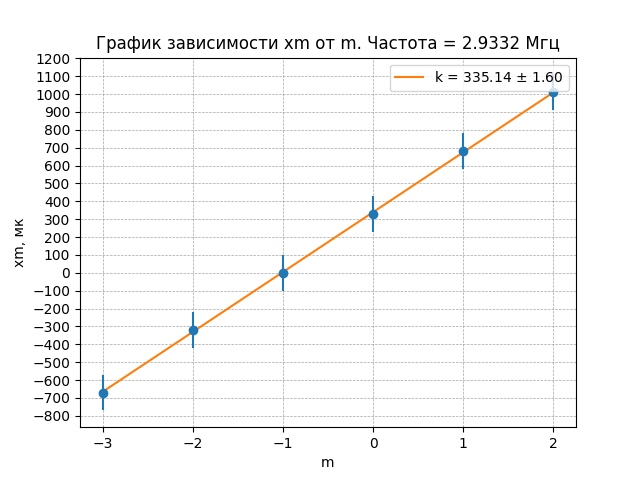
\includegraphics[width=1\textwidth]{3.png}
		\caption{График зависимости $x_{m}(m)$ при $\nu_{3}$}
		\label{diff}
	\end{figure}
	По составленным таблицам и коэффициентам наклона графика определим для каждой частоты $k$, чтобы по формуле (4) рассчитаем длины волн $\Lambda$ для всех частот.
	\begin{center}
	    \begin{tabular}{|c|c|c|c|c|c|}
	         \hline
	         $\nu$, МГц & 1,0116 & 1,2092 & 2,9332 & 4{,}6086 & 5{,}1911 \\ \hline
	         $k$, мкм & 117{,}8 & 136 & 335 & 530 & 595 \\ \hline
	         $\sigma k$, мкм &  0.78 & 2.48 & 1.60 & 0 & 1.66 \\ \hline
	         $\Lambda$, мкм & 1630 & 1410 & 573 & 362 & 323 \\ \hline
	         $\Delta\Lambda$, мкм & 50 & 60 & 30 & 13 & 10 \\ \hline
	    \end{tabular}
	\end{center}
	Построили график $\Lambda(1/\nu)$. По коэффициенту наклона определили скорость ультразвука в воде из формулы (5):
	$$v=1620\pm20\text{ м/с}.$$
	Для сравнения табличное значение составляет $v=1490$ м/с.
\begin{figure}[h!]
		\centering	
		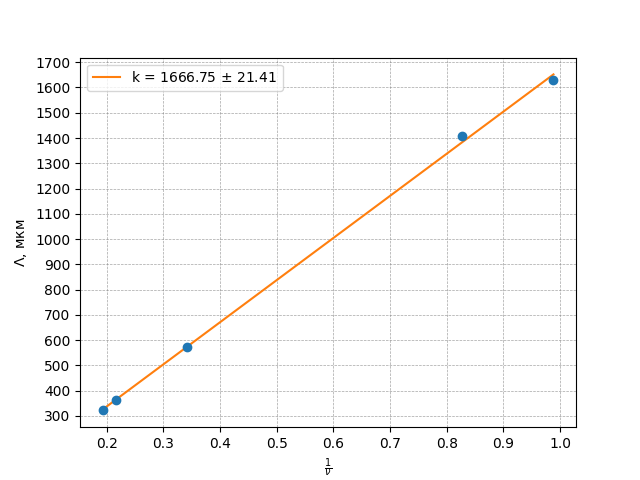
\includegraphics[width=1\textwidth]{4.png}
		\caption{График зависимости $\Lambda(\frac{1}{\nu})$}
		\label{diff}
	\end{figure}
	\newpage
\section*{Определение скорости ультразвука методом темного поля}

Для наблюдения акустической решетки используется метод темного поля, который заключается в устранении центрального дифракционного максимума с помощью непрозрачного экрана. 

Приставим к задней стенке (для светового луча) кюветы стеклянную пластинку с миллиметровыми делениями; сфокусируем микроскоп на изображение пластинки. Определим цену деления окулярной шкалы микроскопа, совместив ее с миллиметровыми делениями: в 6 делениях миллиметровой шкалы убирается 100 маленьких делений окулярной. Значит, цена деления окулярной шкалы: $ C = 0,06 \, \text{мм} $.

Без применения метода темного поля звуковая решетка не наблюдается. Закроем нулевой максимум горизонтальной нитью. Таким образом, осевая составляющая фазово-модулированной волны поглощается, а боковые остаются без изменения. Получившееся поле описывается следующим образом:

\begin{equation}\label{field}
f(x) = \dfrac{im}{2} e^{i\Omega x} +  \dfrac{im}{2} e^{-i\Omega x} = im \cos \Omega x \quad \text{и} \quad I(x) = m^2 \cos^2 \Omega x = m^2 \dfrac{1 + \cos 2\Omega x}{2}
\end{equation}

Отсюда получаем, что расстояние между темными полосами составляет $ \Lambda/2 $.

Проведем измерение длины ультразвуковой волны, приняв ошибку равной цене деления окулярной шкалы. Формулы для расчета длины волны ультразвука $ \Lambda $ и скорости распространения $ v $ в воде:

\begin{equation}\label{wave_speed}
\Lambda/2 = \dfrac{NC}{n - 1}, \quad v = \nu \Lambda
\end{equation}

Расчеты также могут быть представлены в таблице, где содержится количество маленьких делений окулярной шкалы $ N $ (цена деления $ C = 0,06 \, \text{мм} $), соответствующее $ n $ темным полосам акустической решетки. Ошибка при таком определении скорости звука больше, чем в первой части работы. Сами значения тоже получились больше.

	\begin{figure}[h!]
		\centering	
		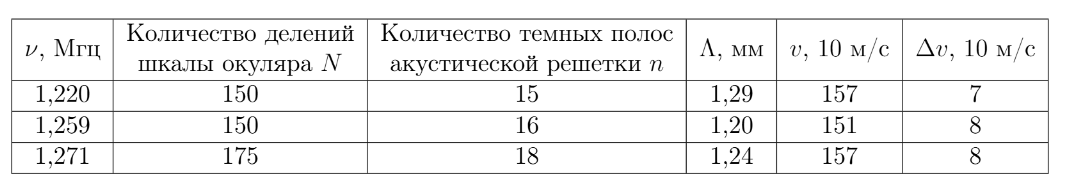
\includegraphics[width=1\textwidth]{5.png}
		\caption{Вычисление длины ультразвуковой волны $\Lambda$ и скорости распространения ее в воде $\upsilon$ методом темного поля.}
		\label{diff}
	\end{figure} 
    \section*{Вывод}
В данной работе была исследована дифракция света на ультразвуковой волне в жидкости. С помощью измерений была определена скорость ультразвука (двумя способами - непосредственно по дифракционной картине и методом тёмного поля). Первый способ позволил достаточно точно определить скорость звука, полученное значение хорошо сошлось с табличным, во втором способе значение получено менее точно из-за больших погрешностей при измерений координат полос, однако всё же сходится с табличным.

\end{document}